%\documentclass[10pt]{beamer}
\documentclass[handout,10pt]{beamer}

\usetheme[progressbar=frametitle]{metropolis}

\usepackage{booktabs}
\usepackage[scale=2]{ccicons}


\usepackage{amsmath}
\usepackage{pgfplots}
\usepgfplotslibrary{dateplot}

\usepackage{xspace}
\newcommand{\themename}{\textbf{\textsc{metropolis}}\xspace}

%\usepackage{placeins} %%%
\usepackage{subfig}
\usepackage{physics}
\usepackage{amssymb}

\usepackage{esint}

\usepackage{tikz}
\usepackage{circuitikz}
\usepackage{siunitx}
\usepackage{tikz-3dplot} %requires 3dplot.sty to be in same directory, or in your LaTeX installation


\usepackage{latexsym}
\usepackage{mathtools}
\usepackage{slashed} % for the Feynman slash notation

\usepackage{listings}

\usepackage{balance}


% edited by Mauro 28-12-16
%
%% <local definitions>
\newcommand{\R}{\mathbb{R}}	
\newcommand{\C}{\mathbb{C}}
\newcommand{\HQ}{\mathbb{H}}
\newcommand{\N}{\mathbb{N}}
\newcommand{\be}{\begin{equation}}
\newcommand{\ee}{\end{equation}}	
\newcommand{\bea}{\begin{eqnarray}}
\newcommand{\eea}{\end{eqnarray}}	
\newcommand{\Pin}{\mathrm{Pin}}	
\newcommand{\Spin}{\mathrm{Spin}}
\renewcommand{\O}{\mathrm{O}}
\newcommand{\SO}{\mathrm{SO}}
\renewcommand{\eqref}[1]{(\ref{#1})}
\newcommand{\cl}[1]{\ensuremath{Cl(#1)}} % #1 stands for the values p,q. $\cl{p,q}$ produces 'Cl(p,q)'.
\newcommand{\gvec}[1]{\ensuremath{\mbox{\textbf{\textit{#1}}}}}
\newcommand{\vect}[1]{\ensuremath{\mbox{\textbf{\textit{#1}}}}}
%% </local definitions>

\newcommand{\Ba}[0]{\mathbf{a}}
\newcommand{\Bb}[0]{\mathbf{b}}
\newcommand{\Bc}[0]{\mathbf{c}}
\newcommand{\Bd}[0]{\mathbf{d}}
\newcommand{\Be}[0]{\mathbf{e}}
\newcommand{\Bf}[0]{\mathbf{f}}
\newcommand{\Bg}[0]{\mathbf{g}}
\newcommand{\Bh}[0]{\mathbf{h}}
\newcommand{\Bi}[0]{\mathbf{i}}
\newcommand{\Bj}[0]{\mathbf{j}}
\newcommand{\Bk}[0]{\mathbf{k}}
\newcommand{\Bl}[0]{\mathbf{l}}
\newcommand{\Bm}[0]{\mathbf{m}}
\newcommand{\Bn}[0]{\mathbf{n}}
\newcommand{\Bo}[0]{\mathbf{o}}
\newcommand{\Bp}[0]{\mathbf{p}}
\newcommand{\Bq}[0]{\mathbf{q}}
\newcommand{\Br}[0]{\mathbf{r}}
\newcommand{\Bs}[0]{\mathbf{s}}
\newcommand{\Bt}[0]{\mathbf{t}}
\newcommand{\Bu}[0]{\mathbf{u}}
\newcommand{\Bv}[0]{\mathbf{v}}
\newcommand{\Bw}[0]{\mathbf{w}}
\newcommand{\Bx}[0]{\mathbf{x}}
\newcommand{\By}[0]{\mathbf{y}}
\newcommand{\Bz}[0]{\mathbf{z}}
\newcommand{\BA}[0]{\mathbf{A}}
\newcommand{\BB}[0]{\mathbf{B}}
\newcommand{\BC}[0]{\mathbf{C}}
\newcommand{\BD}[0]{\mathbf{D}}
\newcommand{\BE}[0]{\mathbf{E}}
\newcommand{\BF}[0]{\mathbf{F}}
\newcommand{\BG}[0]{\mathbf{G}}
\newcommand{\BH}[0]{\mathbf{H}}
\newcommand{\BI}[0]{\mathbf{I}}
\newcommand{\BJ}[0]{\mathbf{J}}
\newcommand{\BK}[0]{\mathbf{K}}
\newcommand{\BL}[0]{\mathbf{L}}
\newcommand{\BM}[0]{\mathbf{M}}
\newcommand{\BN}[0]{\mathbf{N}}
\newcommand{\BO}[0]{\mathbf{O}}
\newcommand{\BP}[0]{\mathbf{P}}
\newcommand{\BQ}[0]{\mathbf{Q}}
\newcommand{\BR}[0]{\mathbf{R}}
\newcommand{\BS}[0]{\mathbf{S}}
\newcommand{\BT}[0]{\mathbf{T}}
\newcommand{\BU}[0]{\mathbf{U}}
\newcommand{\BV}[0]{\mathbf{V}}
\newcommand{\BW}[0]{\mathbf{W}}
\newcommand{\BX}[0]{\mathbf{X}}
\newcommand{\BY}[0]{\mathbf{Y}}
\newcommand{\BZ}[0]{\mathbf{Z}}

\newcommand{\ta}[0]{\tilde{a}}
\newcommand{\tb}[0]{\tilde{b}}
\newcommand{\tc}[0]{\tilde{c}}
\newcommand{\td}[0]{\tilde{d}}

\newcommand{\hA}[0]{\hat{A}}
\newcommand{\hB}[0]{\hat{B}}
\newcommand{\hH}[0]{\hat{H}}

\newcommand{\tA}[0]{\tilde{A}}
\newcommand{\tB}[0]{\tilde{B}}
\newcommand{\tF}[0]{\tilde{F}}
\newcommand{\tE}[0]{\tilde{E}}
\newcommand{\tH}[0]{\tilde{H}}

% spinors definition
\newcommand{\barJ}[0]{\bar{J}}
\newcommand{\barF}[0]{\bar{F}}
\newcommand{\barP}[0]{\bar{P}}
\newcommand{\barW}[0]{\bar{W}}



\newcommand{\tnabla}[0]{\tilde{\nabla}}
\newcommand{\tphi}[0]{\tilde{\phi}}
\newcommand{\tpsi}[0]{\tilde{\psi}}

%
\newcommand{\wavep}[0]{\partial^+}
\newcommand{\wavem}[0]{\partial^-}

\newcommand{\wavepp}[0]{\tilde{\partial}^+}
\newcommand{\wavemp}[0]{\tilde{\partial}^-}

\newcommand{\wavepd}[0]{\bar{\partial}^+}
\newcommand{\wavemd}[0]{\bar{\partial}^-}

\newcommand{\pbd}[0]{\bar{\partial}_d}

% frequency

\newcommand{\helmp}[0]{{\underline{\partial}}^+}
\newcommand{\helmm}[0]{{\underline{\partial}}^-}

\newcommand{\helmpp}[0]{{\underline{\tilde{\partial}}}^+}
\newcommand{\helmmp}[0]{{\underline{\tilde{\partial}}}^-}

\newcommand{\helmpd}[0]{{\underline{\bar{\partial}}}^+}
\newcommand{\helmmd}[0]{{\underline{\bar{\partial}}}^-}

\newcommand{\pbfd}[0]{{\underline{\bar{\partial}}}_d}




\def \figname {Figure}
\def \emode {E }
\def \hmode {H }
\def \temode {TE }
\def \tmmode {TM }
\def \temoden {TE${}_n$ }
\def \tmmoden {TM${}_n$ }
\def \temodemn {TE${}_{mn}$ }
\def \tmmodemn {TM${}_{mn}$ }



\newcommand{\iGA}{{i}}
\newcommand{\conjg}[1] {\ensuremath{#1}^*}

\setbeamertemplate{bibliography item}{[\theenumiv]}


\title{Nabla operator}

\date{}

%\subtitle{Maximizing efficiency and power at a fixed frequency}
%\date{\today}
%\author{Alessandra Costanzo, Franco Mastri, Mauro Mongiardo*, Giuseppina Monti}
%\institute{*Department of Engineering,
%University of Perugia, Italy}

\author{ Mauro Mongiardo$^1$}

\institute{ $^1$ Department of Engineering, University of Perugia, Perugia, Italy.
}

%
\titlegraphic{\hfill\includegraphics[height=1.5cm]{logo}}


\begin{document}

\maketitle

\begin{frame}{Table of contents}
  \setbeamertemplate{section in toc}[sections numbered]
  \tableofcontents[hideallsubsections]
\end{frame}


\def\EMspectrum{\centering
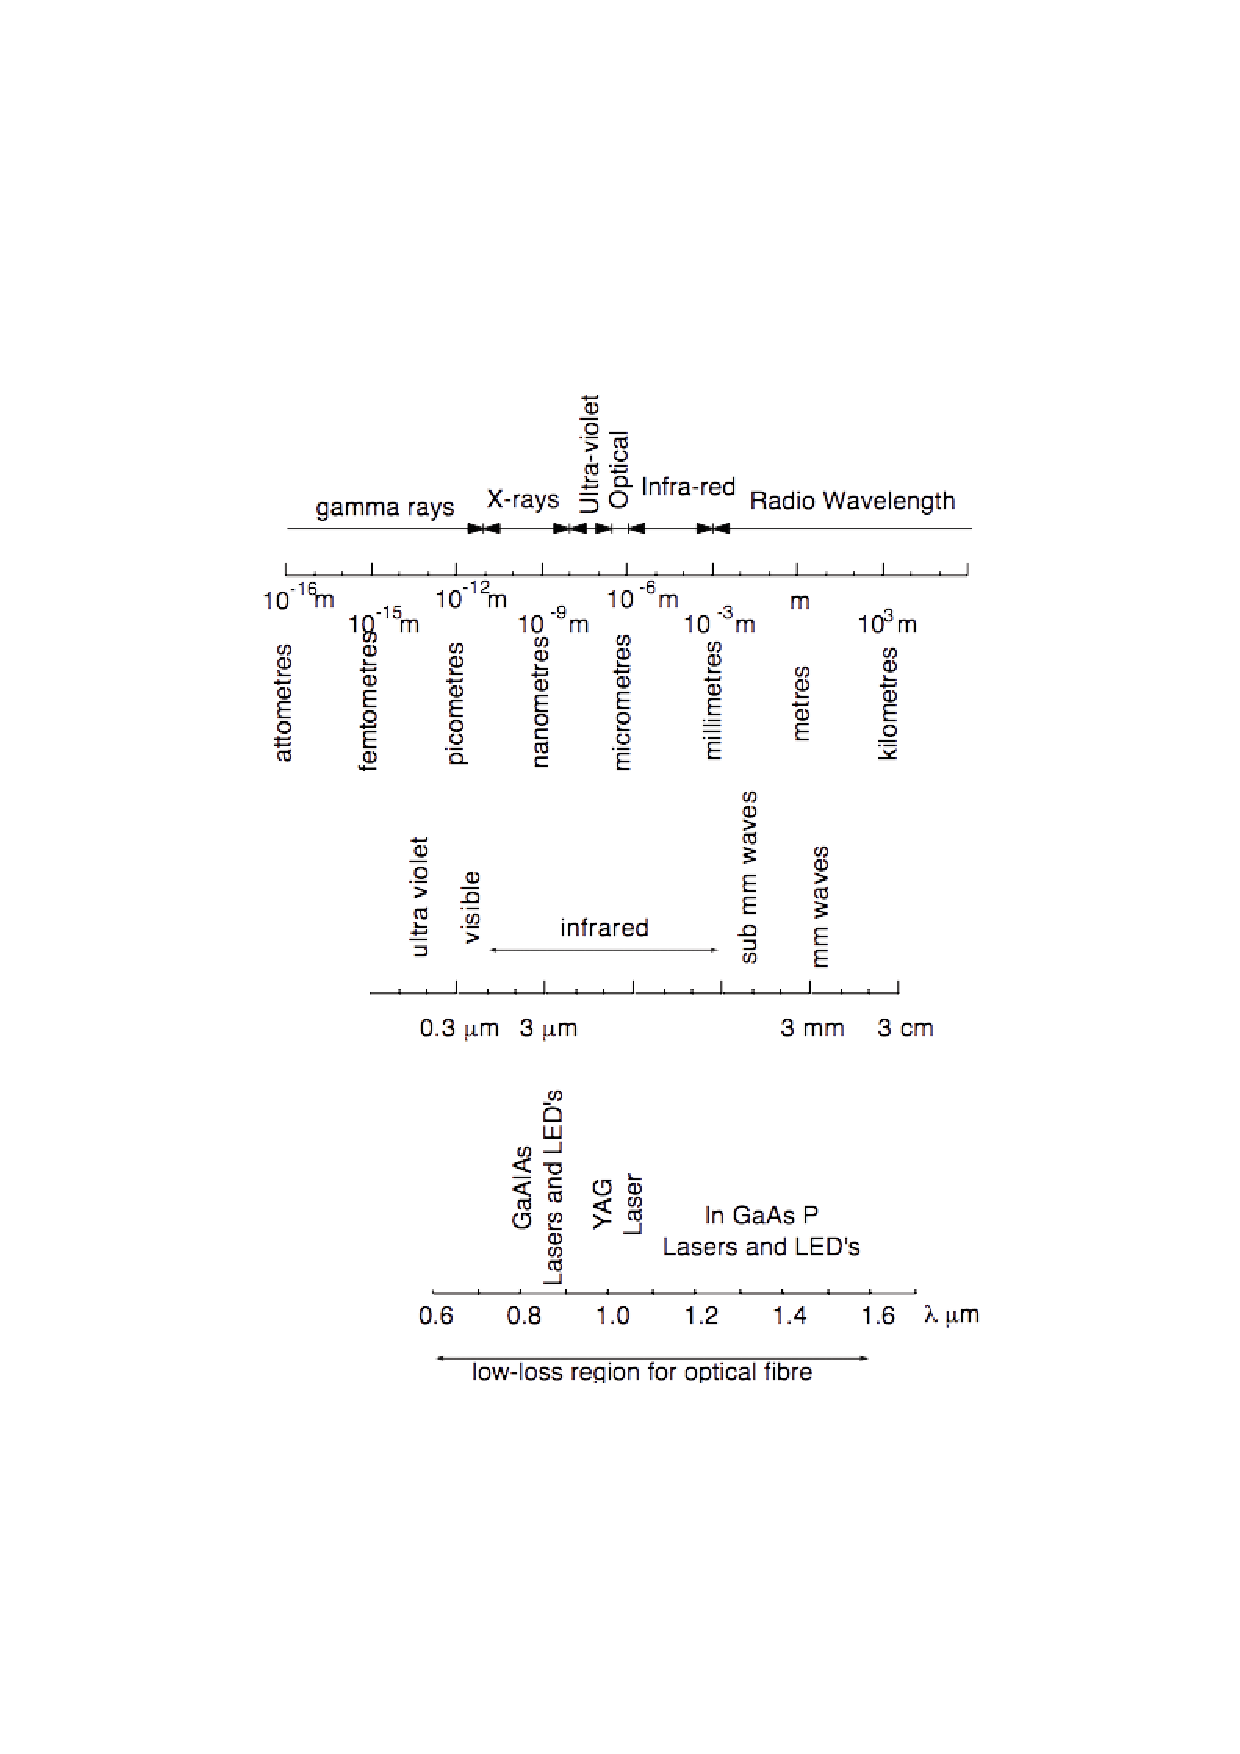
\includegraphics[width=0.75\textwidth]{EMspectrum}}

\def\atmatt{\centering
\includegraphics[width=0.75\textwidth]{atmatt3.eps}}


%



%=========================================================================
\section{Gradient}
%=========================================================================


\begin{frame}[shrink=00]{Gradient definition}
%\subsection{Gradient}


Let us consider a \alert{scalar  function $\phi(\Br)$}, which is single valued and continuous in a volume $V$. 
Physically, the function $\phi$ may represent an electric potential, a temperature, etc. 

At a point $P$ the function will take the value $\phi_P$. 
\pause

Now suppose to \alert{draw a sphere of radius $\Delta s$ centered in $P$}. We can check the values of $\phi(\Br)$ on this sphere and, in general, there will be a point $Q$ on which the variation $\Delta \phi = \phi_P - \phi_Q$ is maximum. 

\pause

This defines also the direction from $P$ to $Q$. This direction is taken as the \alert{direction} of a new vector which is called the \alert{\emph{gradient}}. 

%\pause



\end{frame}

%=========================================================================

\begin{frame}[shrink=00]{Gradient definition}

The magnitude of the gradient is is defined as the value $\Delta \phi/\Delta s$ in this preferred direction. 

\pause

Thus the gradient of a scalar may be defined as 
\be \label{gradient}
grad \phi = \nabla \phi = \Ba_{max} \lim_{\Delta s \to 0} \left( \frac{\Delta \phi}{\Delta s}\right)_{max}
\ee
%
where $\Ba_{max}$ is a unit vector pointing in the direction of maximum $\frac{\Delta \phi}{\Delta s}$.

\pause

\alert{It is noted that the definition (\ref{gradient}) is not dependent on a a particular coordinate system}.
\end{frame}

\begin{frame}[shrink=00]{Gradient in coordinates}
In \alert{rectangular coordinates}, (\ref{gradient}) reduces to
%
\be \label{gradientrect}
 \nabla \phi = \Ba_{x}  \frac{\partial \phi}{\partial x} + \Ba_{y}  \frac{\partial \phi}{\partial y} + \Ba_{z}  \frac{\partial \phi}{\partial z} \, .
\ee
%
\pause
In \alert{circular--cylinder coordinates} , $\Delta s$ in the angular direction $\psi$ is not equal to $\Delta \psi$ but $\delta s = \rho \Delta \psi$. Thus we have
%
\be \label{gradientrect}
 \nabla \phi = \Ba_{\rho}  \frac{\partial \phi}{\partial \rho} + \frac{\Ba_{\psi}}{\rho}  \frac{\partial \phi}{\partial \psi} + \Ba_{z}  \frac{\partial \phi}{\partial z} \, .
\ee
%
\pause
Similarly, in \alert{spherical coordinates}, 
%
\be \label{gradientrect}
 \nabla \phi = \Ba_{r}  \frac{\partial \phi}{\partial r} + \frac{\Ba_{\psi}}{r \sin \theta}  \frac{\partial \phi}{\partial \psi} + \frac{\Ba_{\theta}}{r}  \frac{\partial \phi}{\partial \theta} \, .
\ee
%

\end{frame}

%=========================================================================
\section{Divergence}
%=========================================================================


\begin{frame}{Divergence}

%\subsection{Divergence}
%
Divergence is a scalar function. Let us consider a field, at each point of which a vector $\BF$ is specified. We can associate with each point $P$ a scalar quantity, the divergence of $\BF$, defined as
%
\begin{equation}
div \, {\bf F} = \nabla \cdot {\bf F} = 
\lim_{\Delta \tau \to 0} \frac{1}{\Delta \tau}   \oiint {\bf F}\cdot d{\bf s} \, .
 \label{divdef}
\end{equation}
% Outward flow per unit volume

The point $P$ can be considered enclosed in a surface $\Bs$ of any shape, the volume within the surface being $\Delta \tau$. 
Take the total outward flux of the vector $\BF$ through the bounding surface. The limit of the total outward flux, per unit volume, as the surface shrinks about $P$, is defined as div $\BF$ at the point $P$.

\pause
 In general, div $\BF$ is different for each point in the field.

\end{frame}
%=========================================================================

\begin{frame}[shrink=00]{Divergence in coordinates }

In \alert{rectangular coordinates} the divergence take the following form
%
\begin{equation}
 \nabla \cdot {\bf F} = \frac{\partial F_x}{\partial x} +  \frac{\partial F_y}{\partial y} +  \frac{\partial F_z}{\partial z} \, .
 \label{divdefr}
\end{equation}
%
Equation (\ref{divdefr}) is often used as the definition of divergence. However, since this equation is only valid in rectangular coordinates, it is better to use (\ref{divdef}) as the definition for the divergence.

\pause

In \alert{circular cylindrical coordinates} the divergence has the following expression
%
\begin{equation}
 \nabla \cdot {\bf F} = \frac{1}{\rho} \frac{\partial}{\partial \rho} \left(\rho F_\rho \right) +  
\frac{1}{\rho}  \frac{\partial F_\phi}{\partial \phi} +  \frac{\partial F_z}{\partial z} \, .
 \label{divdefc}
\end{equation}
%

\pause

For \alert{spherical coordinates},
%
\begin{equation}
 \nabla \cdot {\bf F} = \frac{1}{r^2} \frac{\partial}{\partial r} \left(r^2 F_r \right) +  
\frac{1}{r \sin \theta}  \frac{\partial }{\partial \theta} \, \left( F_\theta \sin\theta\right) + \frac{1}{r \sin \theta}  \frac{\partial F_\phi}{\partial \phi} \, .
 \label{divdefs}
\end{equation}
%


\end{frame}
%=========================================================================

\begin{frame}[shrink=00]{Divergence evaluation}

In many circumstances it is possible to evaluate the divergence \alert{without calculation}. 

Whenever \alert{physical intuition} indicates that the flux entering $\Delta \tau$
is the same as the flux leaving it, the integral in (\ref{divdef}) must be zero and consequently also the divergence is zero. 

\pause
In \alert{electrostatics}, for example, one visualizes electric flux lines between charges. At any point $P$  in a  region without charges, the integral in  (\ref{divdef}) must be zero, and we can say immediately that $\nabla \cdot \BD=0$  at such a point. Only if there is a charge distribution of density $\rho$ (\si{coulomb} \si{\meter}$^{-3}$) at $P$ we will have $\nabla \cdot \BD=\rho$, i.e. a \alert{measure of the strength of the source} at $P$.

\pause
Similarly, one may say immediately that \alert{for the magnetic field} $\nabla \cdot \BB=0$ always since there are no magnetic charges and the flux lines invariably form closed loops.


\end{frame}
%=========================================================================

\section{Divergence theorem or Gauss theorem}

\begin{frame}[shrink=00]{Divergence theorem or Gauss theorem}
%\subsubsection{Divergence theorem or Gauss theorem}

%\paragraph{Divergence theorem or Gauss theorem.}
%
Let ${\bf A}({\bf r})$ be any vector function of position, continuous
together with its first derivative throughout a volume $V$ bounded by a
surface $S$. The divergence theorem states that

%
\begin{equation}
\oint_{S} {\bf A}({\bf r}) \cdot {\bf n} \; dS =
\int_{V} \nabla \cdot {\bf A}({\bf r})  \; dV
\label{divergenceq}
\end{equation}
%

As a matter of fact the \alert{Gauss theorem is therefore used to define the
divergence}.

\end{frame}

\section{Curl}
%=========================================================================

\begin{frame}[shrink=00]{Curl}

\subsection{Curl}
%
 Consider an incremental element of area $\Delta s$ and denote the unit normal to it by $\Bu_n$. It is possible to define the vector curl $\BF$, represented symbolically as $\nabla \times {\bf F}$, as
 
\begin{equation}
curl \, {\bf F} = \nabla \times {\bf F} = \lim_{\Delta s \to 0} \frac{1}{\Delta s}   \left[{\bf u}_n  \oint {\bf F}\cdot d{\bf l} \right]_{max} \, .  \label{curldef}
\end{equation}

%maximum circulation per unit area
Note that in general we should repeat this procedure for three orthogonal surfaces and sum their contributions. 

However, assuming assuming to know the direction of the curl (i.e. considering the surface such that the result is max), we can use the above expression.

\end{frame}

%=========================================================================

\begin{frame}[shrink=00]{Curl Expressions}
In rectangular coordinates the curl takes the following form:
%
\begin{equation}
 \nabla \times {\bf F} = 
{\bf u}_x \left(\frac{\partial {F}_{z}}{\partial\,y}\,-\frac{\partial {F}_{y}}{\partial\,z}\right) 
 + {\bf u}_y \left(\frac{\partial {F}_{x}}{\partial\,z}\,-\frac{\partial {F}_{z}}{\partial\,x} \right) 
 +  {\bf u}_z \left(\frac{\partial {F}_{y}}{\partial\,x}\,-\frac{\partial {F}_{x}}{\partial\,y}\right) \, .
 \label{curldefr}
\end{equation}
%
The above expressions can be easily memorized by forming a determinant with the versors on the first line, the partial derivatives on the second line and the vector itself on the third line.

For cylindrical coordinates, the following expression holds:
%
\begin{eqnarray}
 \nabla \times {\bf F} & =  &
{\bf u}_\rho \left( \frac{1}{\rho} \frac{\partial {F}_{z}}{\partial\,\phi}\,-\frac{\partial {F}_{\phi}}{\partial\,z}\,\right) \nonumber \\
& & + {\bf u}_\phi \left(\frac{\partial \,{F}_{\rho}}{\partial\,z}-\frac{\partial \,{F}_{z}}{\partial\,\rho}\right)  \nonumber \\
& &  +  {\bf u}_z \left[ \frac{1}{\rho}  \frac{\partial }{\partial\,\rho}\,\left( \rho {F}_{\phi}\right) -  \frac{1}{\rho} \frac{\partial \,{F}_{\rho}}{\partial\,\phi}\right]
 \label{curldefc}
\end{eqnarray}
%

For spherical coordinates:
%
\begin{eqnarray}
 \nabla \times {\bf F} & =  &
{\bf u}_r  \, \frac{1}{r \sin \theta} \, \left[ \frac{\partial}{\partial \theta} \left( F_\phi \sin \theta\right)  - \frac{\partial F_\theta}{\partial \phi} \right]
\nonumber  \\
& &  +  {\bf u}_\theta \, \frac{1}{r} \, \left[  \frac{1}{\sin\theta} \frac{\partial F_r}{\partial\,\phi} -  \frac{\partial }{\partial\,r} \left( r F_\theta\right)\right] \nonumber  \\
& & + {\bf u}_\phi \, \frac{1}{r} \, \left[ \frac{\partial }{\partial\,r}\left( r F_\theta \right)-\frac{\partial \,{F}_{r}}{\partial\,\theta}\right] 
 \label{curldefs}
\end{eqnarray}
%


\end{frame}
%=========================================================================

\section{Curl theorem or Stokes theorem}
\begin{frame}[shrink=00]{Curl theorem or Stokes theorem}

%\paragraph{Curl theorem or Stokes theorem.}
Let ${\bf A}({\bf r})$ be any vector function of position, continuous
together with its first derivative throughout an arbitrary surface $S$
bounded by a contour $C$, assumed to be resolvable into a finite number
of regular arcs. 

%\pause

The \alert{Stokes theorem} states that
%
\begin{equation}
\oint_{C} {\bf A}({\bf r}) \cdot d{\bf \ell}  =
\int_{S} \left[ \nabla \times {\bf A}({\bf r})\right]
\cdot {\bf n} \; dS
\label{curleq}
\end{equation}
%
where $d{\bf \ell}$ is an element of length along $C$ and ${\bf n}$ is a
unit vector normal to the positive side of the element area $dS$.

This relationship is  an equation defining the
curl.


\end{frame}
%=========================================================================

\section{Scalar Laplacian}
\begin{frame}[shrink=00]{Scalar Laplacian}

The scalar Laplacian is a second order operator, corresponding to the notation $\nabla \cdot \nabla w$  or div grad $w$, that is we have to take the divergence of the gradient of $w$ 
%
\begin{equation}
div \,(grad \, w) = \nabla^2 w = \nabla \cdot \nabla w
 \label{Laplacian}
\end{equation}
%
\pause
In the following are reported the Laplacian expressions in cartesian, circular-cylindrical and spherical coordinate systems, respectively.
%
\begin{equation}
 \nabla^2 w =  \frac{\partial^2 w}{\partial x^2} +  \frac{\partial^2 w}{\partial y^2} +  \frac{\partial^2 w}{\partial z^2} 
 \label{Laplacianr}
\end{equation}
%
\pause
%
\begin{equation}
 \nabla^2 w =  \frac{1}{\rho} \frac{\partial }{\partial\,\rho}\,\left( \rho \frac{\partial w}{\partial \rho} \right) + 
 \frac{1}{\rho^2} \frac{\partial^2 w}{\partial \phi^2} +  \frac{\partial^2 w}{\partial z^2} 
 \label{Laplacianc}
\end{equation}
%
\pause
%
\begin{equation}
  \nabla^2 w  = \frac{1}{r^2}\frac{\partial}{\partial r}\left(r^2  \frac{\partial w}{\partial r}\right)  +   
 \frac{1}{r^2 \sin \theta}   \frac{\partial}{\partial \theta}  \left(  \sin \theta\frac{\partial w}{\partial \theta} \right) 
+  \frac{1}{r^2 \sin^2 \theta}\frac{\partial^2 w}{\partial \phi^2}  
  \label{Laplacians}
\end{equation}
%


\end{frame}

\section{Summary}
\begin{frame}[shrink=00]{Rectangular coordinates}



%
\begin{equation}
 \nabla w = {\bf u}_x \frac{\partial w}{\partial x} + {\bf u}_y \frac{\partial w}{\partial y} + {\bf u}_z \frac{\partial w}{\partial z} 
  \label{graddefr}
\end{equation}
%


%
\begin{equation}
 \nabla \cdot {\bf F} = \frac{\partial F_x}{\partial x} +  \frac{\partial F_y}{\partial y} +  \frac{\partial F_z}{\partial z}
 \label{divdefr}
\end{equation}
%



%
\begin{equation}
 \nabla \times {\bf F} = 
{\bf u}_x \left(\frac{\partial {F}_{z}}{\partial\,y}\,-\frac{\partial {F}_{y}}{\partial\,z}\right) 
 + {\bf u}_y \left(\frac{\partial {F}_{x}}{\partial\,z}\,-\frac{\partial {F}_{z}}{\partial\,x} \right) 
 +  {\bf u}_z \left(\frac{\partial {F}_{y}}{\partial\,x}\,-\frac{\partial {F}_{x}}{\partial\,y}\right)
 \label{curldefr}
\end{equation}
%



%
\begin{equation}
 \nabla^2 w =  \frac{\partial^2 w}{\partial x^2} +  \frac{\partial^2 w}{\partial y^2} +  \frac{\partial^2 w}{\partial z^2} 
 \label{Laplacianr}
\end{equation}
%

\end{frame}


\begin{frame}[shrink=00]{Cylindrical coordinates}

%\subsection{Cylindrical coordinates}


%
\begin{equation}
 \nabla w = {\bf u}_\rho \frac{\partial w}{\partial \rho} + {\bf u}_\phi \frac{1}{\rho} \frac{\partial w}{\partial \phi} + {\bf u}_z \frac{\partial w}{\partial z} 
  \label{graddefc}
\end{equation}
%


%
\begin{equation}
 \nabla \cdot {\bf F} = \frac{1}{\rho} \frac{\partial}{\partial \rho} \left(\rho F_\rho \right) +  
\frac{1}{\rho}  \frac{\partial F_\phi}{\partial \phi} +  \frac{\partial F_z}{\partial z}
 \label{divdefc}
\end{equation}
%



%
\begin{eqnarray}
 \nabla \times {\bf F} & =  &
{\bf u}_\rho \left( \frac{1}{\rho} \frac{\partial {F}_{z}}{\partial\,\phi}\,-\frac{\partial {F}_{\phi}}{\partial\,z}\,\right) \nonumber \\
& & + {\bf u}_\phi \left(\frac{\partial \,{F}_{\rho}}{\partial\,z}-\frac{\partial \,{F}_{z}}{\partial\,\rho}\right) \nonumber \\
& &  +  {\bf u}_z \left[ \frac{1}{\rho}  \frac{\partial }{\partial\,\rho}\,\left( \rho {F}_{\phi}\right) -  \frac{1}{\rho} \frac{\partial \,{F}_{\rho}}{\partial\,\phi}\right]
 \label{curldefc}
\end{eqnarray}
%


%
\begin{equation}
 \nabla^2 w =  \frac{1}{\rho} \frac{\partial }{\partial\,\rho}\,\left( \rho \frac{\partial w}{\partial \rho} \right) + 
 \frac{1}{\rho^2} \frac{\partial^2 w}{\partial \phi^2} +  \frac{\partial^2 w}{\partial z^2} 
 \label{Laplacianc}
\end{equation}
%



\end{frame}

\begin{frame}[shrink=00]{Spherical coordinates}
%\subsection{Spherical coordinates}


%
\begin{equation}
 \nabla w = {\bf u}_r \frac{\partial w}{\partial r} +   {\bf u}_\theta \frac{1}{r} \frac{\partial w}{\partial \theta} + {\bf u}_\phi \frac{1}{r \sin \theta} \, \frac{\partial w}{\partial \phi} 
  \label{graddefs}
\end{equation}
%


%
\begin{equation}
 \nabla \cdot {\bf F} = \frac{1}{r^2} \frac{\partial}{\partial r} \left(r^2 F_r \right) +  
\frac{1}{r \sin \theta}  \frac{\partial }{\partial \theta} \, \left( F_\theta \sin\theta\right) + \frac{1}{r \sin \theta}  \frac{\partial F_\phi}{\partial \phi}
 \label{divdefs}
\end{equation}
%



%
\begin{eqnarray}
 \nabla \times {\bf F} & =  &
{\bf u}_r  \, \frac{1}{r \sin \theta} \, \left[ \frac{\partial}{\partial \theta} \left( F_\phi \sin \theta\right)  - \frac{\partial F_\theta}{\partial \phi} \right]
\nonumber \\
& &  +  {\bf u}_\theta \, \frac{1}{r} \, \left[  \frac{1}{\sin\theta} \frac{\partial F_r}{\partial\,\phi} -  \frac{\partial }{\partial\,r} \left( r F_\phi\right)\right] \nonumber \\
& & + {\bf u}_\phi \, \frac{1}{r} \, \left[ \frac{\partial }{\partial\,r}\left( r F_\theta \right)-\frac{\partial \,{F}_{r}}{\partial\,\theta}\right] 
 \label{curldefs}
\end{eqnarray}
%


%
\begin{equation}
  \nabla^2 w  = \frac{1}{r^2}\frac{\partial}{\partial r}\left(r^2  \frac{\partial w}{\partial r}\right)  +   
 \frac{1}{r^2 \sin \theta}   \frac{\partial}{\partial \theta}  \left(  \sin \theta\frac{\partial w}{\partial \theta} \right) 
+  \frac{1}{r^2 \sin^2 \theta}\frac{\partial^2 w}{\partial \phi^2}  
  \label{Laplacians}
\end{equation}
%

\end{frame}

\section{Vector operation with CAS}

\begin{frame}[shrink=00]{Vector operation with CAS: Cartesian coordinates}
%\subsection{Vector operation with CAS: Cartesian coordinates}
 
  
%\subsubsection{Cartesian coordinates} 
A code for performing vector algebra with wxMaxima in cartesian coordinates is reported next.
 With small modifications the code can be used to compute divergence gradient curl etc. of specific functions.

%\newpage
\small
\lstinputlisting{vect_op_rectangular.wxm}
\normalsize
\newpage

\subsection{Cylindrical coordinates} 

%\newpage
\small
\lstinputlisting{vect_op_cyl.wxm}
\normalsize
\newpage


\end{frame}

\begin{frame}[shrink=00]{Vector operation with CAS: Cylindrical coordinates}
%\subsection{Cylindrical coordinates} 

%\newpage
\small
\lstinputlisting{vect_op_cyl.wxm}
\normalsize
\newpage

\end{frame}


\begin{frame}[shrink=00]{Vector operation with CAS: Spherical coordinates}

%\subsection{Spherical coordinates} 

%\newpage
\small
\lstinputlisting{vect_op_spherical.wxm}
\normalsize
\newpage

\end{frame}

%\begin{frame}[shrink=00]{}
%\end{frame}
%
%\begin{frame}[shrink=00]{}
%\end{frame}
%
%\begin{frame}[shrink=00]{}
%\end{frame}
%
%\begin{frame}[shrink=00]{}
%\end{frame}
%
%\begin{frame}[shrink=00]{}
%\end{frame}
%
%\begin{frame}[shrink=00]{}
%\end{frame}
%
%\begin{frame}[shrink=00]{}
%\end{frame}


%\begin{frame}[shrink=20]{Coordinate systems}
%\end{frame}
%\begin{frame}[shrink=20]{Coordinate systems}
%\end{frame}
%
%\begin{frame}[shrink=20]{Coordinate systems}
%\end{frame}
%
%\begin{frame}[shrink=20]{Coordinate systems}
%\end{frame}
%
%\begin{frame}[shrink=20]{Coordinate systems}
%\end{frame}
%
%\begin{frame}[shrink=20]{Coordinate systems}
%\end{frame}
%
%\begin{frame}[shrink=20]{Coordinate systems}
%\end{frame}
%
%\begin{frame}[shrink=20]{Coordinate systems}
%\end{frame}
%
%\begin{frame}[shrink=20]{Coordinate systems}
%\end{frame}
%
%\begin{frame}[shrink=20]{Coordinate systems}
%\end{frame}
%
%\begin{frame}[shrink=20]{Coordinate systems}
%\end{frame}
%
%\begin{frame}[shrink=20]{Coordinate systems}
%\end{frame}



\end{document}
